%%% Preamble
\documentclass[paper=a4, fontsize=11pt]{scrartcl}
\usepackage[T1]{fontenc}
\usepackage{fourier}
\usepackage[brazilian]{babel}							% Português
\usepackage[protrusion=true,expansion=true]{microtype}	
\usepackage{amsmath,amsfonts,amsthm} % Math packages
\usepackage[pdftex]{graphicx}
\usepackage{graphicx}	
\usepackage{url}
\usepackage{indentfirst}
\usepackage{mathtools}
\usepackage{listings}
\DeclarePairedDelimiter{\Vector}{\lparen}{\rparen}

%%% Custom sectioning
\usepackage{sectsty}
\allsectionsfont{\centering \normalfont\scshape}


%%% Custom headers/footers (fancyhdr package)
\usepackage{fancyhdr}
\pagestyle{fancyplain}
\fancyhead{}											% No page header
\fancyfoot[L]{}											% Empty 
\fancyfoot[C]{}											% Empty
\fancyfoot[R]{\thepage}									% Pagenumbering
\renewcommand{\headrulewidth}{0pt}						% Remove header underlines
\renewcommand{\footrulewidth}{0pt}						% Remove footer underlines
\setlength{\headheight}{13.6pt}

%%% Maketitle metadata
\newcommand{\horrule}[1]{\rule{\linewidth}{#1}} 		% Horizontal rule

\title{
		%\vspace{-1in} 	
		\usefont{OT1}{bch}{b}{n}
		\normalfont \normalsize \textsc{Insper: Instituto de Ensino e Pesquisa} \\ [25pt] %Instituição
		\horrule{0.5pt} \\[0.4cm]														  
		\huge Implementação e análise de treliças planas \\			%Título do relatório
		\horrule{2pt} \\[0.5cm]
}
\author{										%Autores
		\normalfont 								\normalsize
        Marcelo Andrade\\[-3pt]		\normalsize
		Pedro Cunial\\[-3pt]		\normalsize
        Gabriela Almeida\\[-3pt]		\normalsize
}
\date{\today}


%%% Início document
\begin{document}
	
%%% Capa do documento
\maketitle

\newpage

%% Sumário
\tableofcontents

\newpage

%%% Início Relatorio

%%% Objetivos
\section{Objetivos}
Os objetivos do projeto são os seguintes:

\begin{itemize}
	\item Implementar um programa para análise de tração/compressão em
	treliças planas. O código deverá ser escrito de modo que os dados de entrada
	possam ser facilmente alterados a partir de um arquivo de texto. O programa deverá gerar um arquivo de saída.
	
	\item Aplicar técnicas numéricas e implementar um programa para
	solução de sistemas de equações. 
	
	\item Analisar o arquivo de saída com o pós-processamento dos dados
	disponibilizado. 
\end{itemize}

%%% Introdução
\section{Introdução}

%%% Metodologia
\section{Metodologia}

A partir do arquivo de entrada do programa, primeiramente calcula-se os graus de liberdade de cada um dos elementos a partir da matriz de incidências do arquivo de entrada. Sendo \(N\) os graus de liberdade de um elemento \(x\), e \(I\) a matriz de incidências:


\[N_x = 
\begin{bmatrix}
I_{x1} - 1 ,& I_{x1} ,& I_{x2} - 1 ,& I_{x2}  \\
\end{bmatrix}
\]

Em seguida, calcula-se as especificações de cada elemento da treliça a partir da matriz de coordenadas \(C\), sendo elas o comprimento do elemento, cosseno e seno do ângulo. Considerando\(L\) o comprimento do elemento \(x\), \(cos\) o cosseno do ângulo \(\theta\) de \(x\) e \(sin\) o seno do ângulo \(\theta\) de \(x\):

\[L_x = \sqrt{(x_2 - x_1)^2 + (y_2 - y_1)^2}\]

\[sin_x = \frac{y_2 - y_1}{L_x}\]

\[cos_x = \frac{x_2 - x_1}{L_x} \]

Com as especificações de cada elemento obtidas, calcula-se as matriz de rigidez do elemento de barra no sistema global, representada por \(K_e\). Sendo \(E\) o módulo de elasticidade do material da barra, \(A\) a área da seção transversal da barra, \(l\) o comprimento da mesma e \(c\) e \(s\) respectivamente o cosseno e seno do ângulo \(\theta\) do elemento:

\[K_e = \frac{E \cdot A}{l}
\begin{bmatrix}
c^2 & cs & -c^2 & -cs\\
cs & s^2 & -cs & -s^2 \\
-c^2 & -cs & c^2 & cs \\
-cs & -s^2 & cs & s^2
\end{bmatrix}
\]

Já com a matriz de rigidez no sistema global de cada elemento, calculou-se a matriz de rigidez global da treliça, representada por \(K_g\). Para esse cálculo, primeiro tem-se que determinar as matrizes de superposição para cada elemento, a soma dessas matrizes resulta na rigidez global da treliça. 
	
As matrizes de superposição são obtidas através substituição dos índices da matriz \(K_e\) pelos seus respectivos graus de liberdade.

A partir da matriz \(K_g\), utilizando o vetor de forças globais e os graus de liberdade dos nós, aplica-se as condições de contorno na matriz \(K_g\).

Com a matriz \(K_g\) simplificada para a análise e a usando a matriz de forças \(P_g\), foi-se calculado o vetor de deslocamento dos nós da treliça, representada por \(U\).

\[[K_g]\cdot\{U\} = \{P_g\}\]

Pode-se interpretar a equação matricial acima como um sistema de equações. Utilizou-se o método numérico de Gauss-Seidel, como é explicado em \cite{gauss_seidel}. Usamos como entrada do método um número máximo de 1000 iterações e um erro esperado igual a 0 com precisão de ponto flutuante, resultando nos valores do vetor de deslocamento.

Com o vetor de deslocamento calculado e utilizando a matriz \(K_g\) anterior as condições de contorno descritas, aplicamos condições de contorno no vetor \(U\) e na matriz \(K_g\) e determinou-se as reações de apoio em cada um dos nós da treliça, formando uma matriz \(R\) de reações.

\[\{R\} = [K_g] \{U\}\]

Por fim, calculou-se a tensão e deformação de cada um dos elementos, a tensão representado por \(\sigma\) e a deformação representada por \(\epsilon\).

\[\sigma = \frac{E}{l}  
\begin{bmatrix}
-c & -s & c & s\\
\end{bmatrix}
\begin{bmatrix}
u_1 \\
v_1 \\
u_2 \\
v_2 \\
\end{bmatrix}
\]


\[\epsilon = \frac{1}{l}  
\begin{bmatrix}
-c & -s & c & s\\
\end{bmatrix}
\begin{bmatrix}
u_1 \\
v_1 \\
u_2 \\
v_2 \\
\end{bmatrix}
\]

Com todos os valores das reações de apoio, tensões e deformações dos elementos, e deslocamentos dos nós, exportou-se todos os dados em um arquivo de saída.

%%% Resultados e Discussão
\section{Resultados e Discussão}


\begin{figure}[!htb]
	\centering
	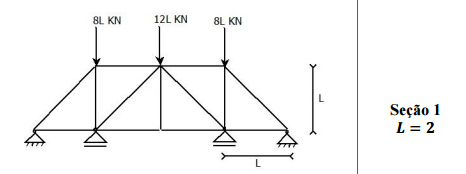
\includegraphics{trelica_entrada.png}
	\caption{Figura representativa da entrada do programa}
	\label{Rotulo}
\end{figure}

\begin{figure}[!htb]
	\centering
	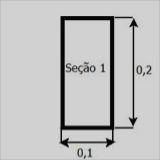
\includegraphics{secao1.png}
	\caption{Seção usada na entrada}
	\label{Rotulo}
\end{figure}


%%% Conclusões
\section{Conclusões}

%%% Agradecimentos
\section{Agradecimentos} 


\bibliography{referencias}{}
\bibliographystyle{plain}

%%% Fim do Documento
\end{document}